\chapter{Periodic table and energy}
	The focus of this module is inorganic and physical chemistry, the applications of energy use to everyday life and industrial processes, and current environmental concerns associated with sustainability. 

\section{The Periodic table 3.1.1}
	
	\paragraph{Simply put} the periodic table lists the known elements in order of atomic number\footnote{A number derived from the number of protons} 
    \paragraph{Periodicity is} when periods show repeating trends
in \textbf{physical and chemical} properties. This section focuses on periodicity of the following properties: elec.config., ionisation energy, structure and melting points.
\paragraph{In period 2} the highest orbital sub-shell filled are the 2s and 2p ones. In \textbf{period 3}, the highest are the 3s and 3p sub-shells. In \textbf{period 4}, the 3d subshell is filled as well as the 4s and 4p subshells only.\footnote{Important to remember as it cuts down time in exam.}

	
	\paragraph{Groups, or vertical columns}, generally contain chemicals of similar properties.
	This is because they all have the same amount of electrons missing in the outer shell\footnote{Sort of true for first three periods}. 
    Periods or horizontal rows gives the number of the highest energy electron shell in an element's atoms
	\subsection*{Ionisation energies}
	\paragraph{First ionisation energy} is the amount of \textbf{energy required to remove one electron} from \textbf{each atom} in \textbf{one mole} of \textbf{gaseous} substance.There are several things which affect first ionisation energy which I will now go into.
    e.g. \ch{Na_{(g)} -> Na$^+$_{(g)} + e$^-$}
	\paragraph{The first ionisation energy} generally \textbf{increases as we go across the period and decreases as we go down} the group in general.This is because as we move \textbf{across the period the nuclear charge gets greater}.
This then affects the \textbf{atomic radius, making it smaller}.This means that the \textbf{electrons on the outer shells} are \textbf{more attracted to the nucleus} and so the first ionisation energy increases.( revert back to definition if you don't understand)..

\subsection*{Factors affecting ionisation energies}
\paragraph{1. Atomic radius-}the greater the distance, the less attraction to the outer electron, decreasing ionisation energy.
\paragraph{2. Nuclear charge-}if there are \textbf{more protons} and therefore electrons, the \textbf{attraction} between the nucleus and electrons is \textbf{higher}. This makes the atomic radius smaller,thus increasing first ionisation energy.
\paragraph{3. Electron shielding-}as electrons are -ve charged, the \textbf{inner electrons repel outer electrons}. This is called the \textbf{shielding effect}. It reduces the attraction between the nucleus and outer electrons, reducing first ionisation energy.
\subsubsection*{Successive ionisation energies}	
\paragraph{An element has as many ionisation energies as its number of electrons.}This means that as you go down a group, there are more ionisation energies. For example helium has 2 electron, so:
 \ch{He_{(g)} -> He$^+$_{(g)} + e$^-$} and
 \ch{He^+$_{(g)} -> He$^{2+}_{(g)} + e$^-$}.
 \paragraph{The second ionisation energy of helium} is much greater than than the first because there are two protons attracting two electrons. When an electron is removed, the single electron is more strongly attracted to the nucleus. This increases the ionisation energy.
 \paragraph{The second ionisation energy is the}amount of energy required to remove 1 electron from each atom in a +1 ion of a gaseous element to form 2+ ions.
 \subsubsection{Successive ionisation energies and shells}
 \begin{center}
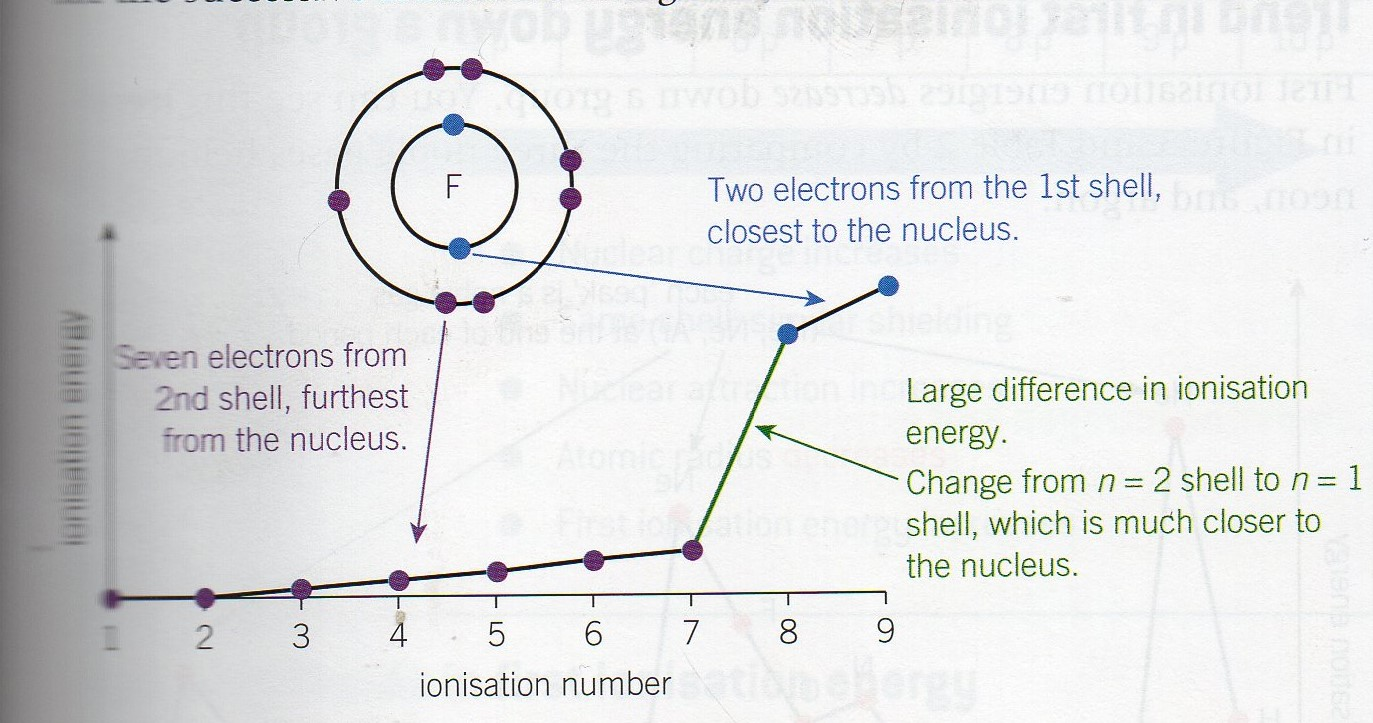
\includegraphics[scale=1]{ionisatione}
\end{center}
\paragraph{The large increase between the 7th and 8th}ionisation energies can be explained by the 1s shell being reached, which has the strongest attraction to the nucleus. This means that more energy is needed to remove electrons in this subshell.
\paragraph{You can make predictions from the successive ionisation energies.} These are the group of the element, the number of electrons in the outer shell and the identity of the element.
\subsection{Trends in ionisation energies}
\paragraph{There is a general increase in ionisation energies across a period.}However, there is a sharp decrease in first ionisation energy between the end of a period and the start of a new one(noble gases are peaks).
\begin{center}
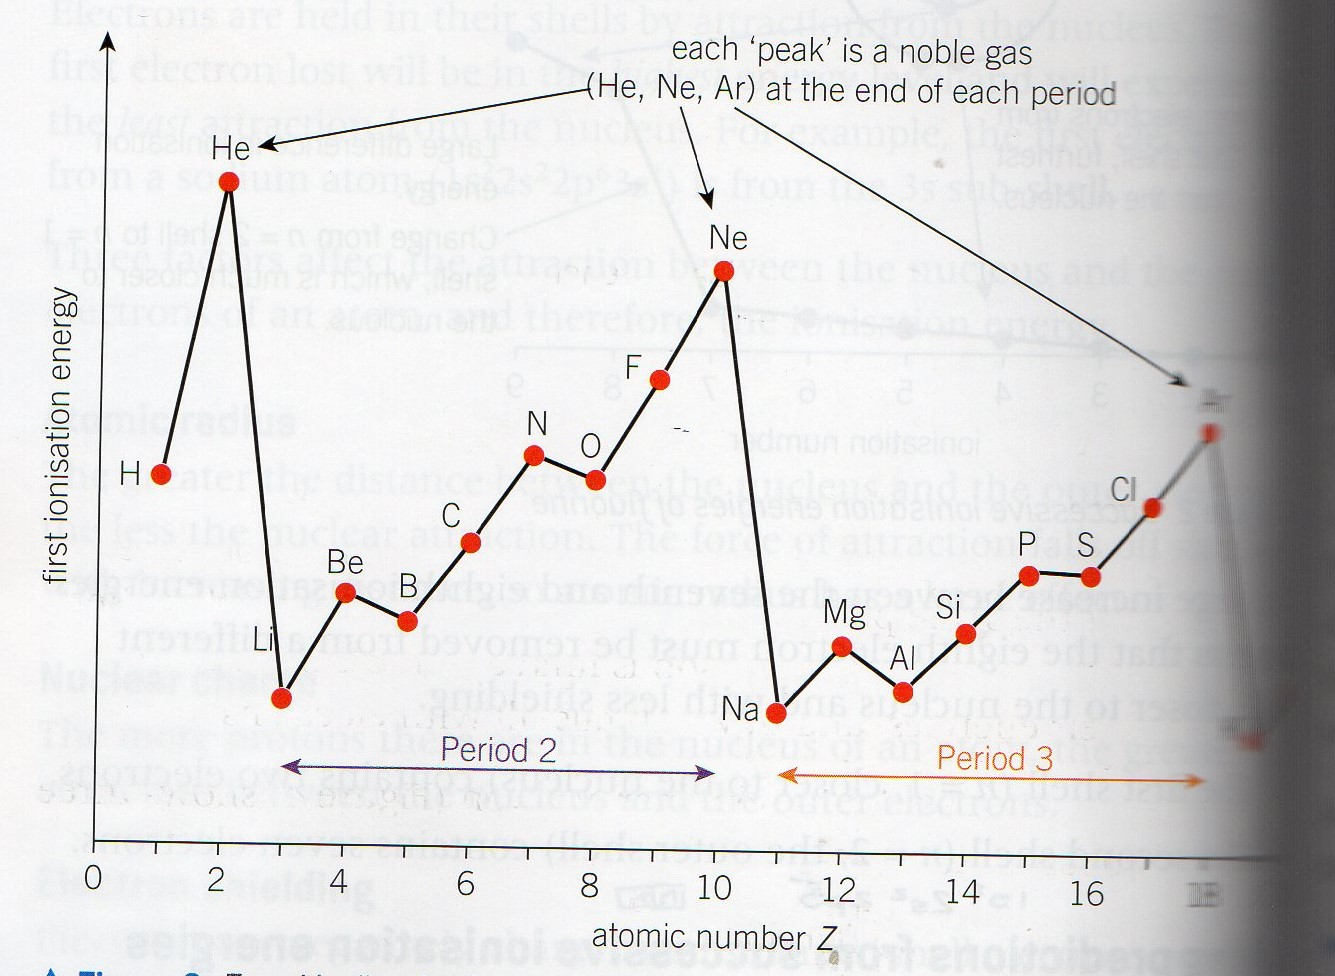
\includegraphics[scale=0.7]{periodio}
\end{center}
\paragraph{First ionisation energy decreases down all groups}because the atomic radius increases and electron shielding increases. Although nuclear charge increases, these effects outweigh it. 
\paragraph{First ionisation energy increases across periods.}This is due to similar levels of electron shielding as they are in the same shell.Next, there is a greater nuclear charge, increasing nuclear attraction as the atomic radius is smaller. This means that it is harder to remove electrons form elements.
\paragraph{Electrons in the same p sub-orbital repel each other. This makes it easier to remove an electron, decreasing first ionisation energy e.g. with N and O.}
\section{Periodic trend in structure 3.1.1}
	
	\paragraph{Metallic bonding} is the a ``strong electrostatic attraction between \textbf{fixed} cations (positive ions) and a sea of \textbf{delocalised} electrons".
	This bonding is between metal atoms and forms giant metallic lattices.
	\paragraph{Metals are able to conduct electricity} because of the sea of delocalised electrons created each metal donating its electrons to a shared pool of electrons.
	Metals are almost always \textbf{solid} at room temperature, except for mercury.
	This is because \textbf{metallic bonding is very strong}, but dependent on how many electrons the elements lose i.e. how positive cations are, as well as well as other factors.
    \paragraph{The melting point of metallic structures} is dependant upon the strength of the electrostatic attraction between cations and electrons. 
    Metals do not dissolve. This is even true with polar solvents as metals react rather than dissolving.
	
	\paragraph{Giant covalent lattices} are, unlike simple molecular lattices, atoms not molecules bonded by covalent bonds.
	This can make for some \textbf{incredibly strong compounds}.
	Carbon, boron and silicon are examples of atoms that can form giant covalent lattices.
	Carbon can form Diamond, graphite and graphene.
    \paragraph{Other than graphite and graphene, giant covalent lattices will not conduct electricity.}
	This is because the electrons are \textbf{immobile}. However graphite has a free electron per carbon atom. 
	These electrons join a sea of delocalised electrons and can move between the layers in the carbon.
	These mobile charge carriers are what allow graphite and graphene to be conductive.
	
	\paragraph{Solubility} Both metals and giant covalent lattices are, on the whole insoluble.
	In the case of metals, they may well react when in polar solvents not dissolve.
	In the case of giant covalent lattices, the bonding is far too strong to be broken by solvents.
	
	\paragraph{Graphene} is the latest wonder allotrope of carbon.
	It consists of a single layer of graphite, composed of hexagonally linked carbon atoms.
	It has the same electrical conductivity of copper and is the thinnest, strongest element ever made.
	The reason for its electrical conductivity is that it has, like graphite, delocalised electrons- as it doesn't use all electrons for bonding.
	These act as mobile charge carriers.
	
	There is potential for this to be used in micro-computing to replace silicone, this could serve to further decrease the size and cost of computer processors.
	
	\paragraph{Melting points} for giant metallic/covalent structures are very high.
	This means the following (for periods 2 and 3):
	\begin{itemize}
		\item As we move from groups 1 to 14 we see a rise in melting temperatures as these elements form \textit{giant structures}.
		\item A sharp drop is seen at group 14 to 15. This is because group 15-18 elements don't form giant structures.
		\item Group 15 to 18 are comparatively low. This is because are \textit{simple molecular structures}.
	\end{itemize}
\section{Group 2 -3.1.2}

	\paragraph{S sub-shell} Is filled in all the group two elements.
	This means that they contain two more electrons than the Nobel gas before it.Note that redox reaction are the most common ones involving Group 2 elements.In redox reactions these substances loose two electrons and from 2+ ions.The next part is just revisiting redox and so I will just summarise.You should know how group two elements from Mg$\rightarrow$Ba react with water, oxygen and weak acids.Just know that group 2 elements are oxidised by +2.
	
	\paragraph{Reactivity} increases as we go down the group because the group two elements in a reaction lose electrons.
	So as we learned before, as we move down the group the first (and in this case second) ionisation energies decrease due to greater shielding\footnote{Shielding is where electrons from other shells repel electrons in the outer shells.} and a greater atomic radius,reducing nuclear attraction.
e.g. \ch{CaO$_{(s)} + H2O$_{(l)}->Ca$^{2+}_{(aq)} + 2 OH$^-_{(aq)}}
\paragraph{Note that alkalinity increases if you shake Group 2 metals in water, going down the group.}This is because the solubility of OH$^-$ ions increases as you go down the group.Also,Ca(OH)2 is used in agriculture to neutralise acid soils and Mg(OH)2 and CaCO3 are used as ‘antacids’ in treating indigestion.
\section{The halogens 3.1.3}
	\paragraph{Boiling trends} in halogens are caused because of there existence as diatomic molecules.
	\textbf{The boiling point increases down the group} because of the \textbf{stronger London forces} (caused by more electrons to allow extra random motion causing induced dipoles).
\paragraph{Redox again} is found here. Much the same as all the others but this time they are oxidising agents.This is because they need only gain one electron to have the electron configuration of a noble gas.They form anions.
	
	\paragraph{Displacement reactions} occur when a significantly \textbf{more reactive chemical} is reacted with a compound containing a similar, but less reactive, compound.Using displacement reactions we can see that reactivity decreases down the group.
\paragraph{Halogen-halide displacement} The reactions are as follows,
	\begin{itemize}
		\item a chloride solution will not be displaced by bromine or iodine. This is because chlorine is the most reactive.
		\item a bromide solution will react when chlorine is added. It will turn orange as the Br$^-$ ions are displaced and so from Br$_2$,
		
			\ch{Cl2(aq) + 2 Br^-(aq) -> 2 Cl^-(aq) + Br2(aq)}
			However given that iodine is less reactive still there will be no reaction between \ch{I2} and bromide.
		\item As the least reactive iodide solution will be displaced by both chlorine and bromine to form a brown solution,
		
			\ch{Cl2(aq) + 2 I^-(aq) -> 2 Cl^-(aq) + I2(aq)}
			
			\ch{Br2(aq) + 2 I^-(aq) -> 2 Br^-(aq) + I2(aq)}
	\end{itemize}
	To tell apart the similar brown and orange we can add a non-polar solvent like cyclohexane to dissolve the halogen.
	When \ch{I2} is dissolved we can see the cyclohexane layer go a deep violet.
	
	\paragraph{The reason for decreasing reactivity} is that it is the opposite to group two.
	To gain an electron we need more attraction.
	As such more shielding and a grater atomic radius just cause less attraction to the electron and make it less reactive.
	
	\paragraph{Disproportionation} is what we call a reaction when the same element undergoes reduction and oxidation.
	This is illustrated by the following,
	\begin{itemize}
		\item The treatment of water with chlorine
		
		\ch{"\ox{0, Cl}" {}2(aq) + H2O(l) -> H "\ox{+1,Cl}" {}O(aq) + H "\ox{-1, Cl}" {}(aq)}
		
		As we can see, Chlorine has been both oxidised and reduced.
		
		\item The reaction of chlorine with cold, dilute aqueous sodium hydroxide,
		
		\ch{"\ox{0, Cl}" {}2(aq) + 2 NaOH(aq) -> Na "\ox{+1, Cl}" {}O(aq) + Na "\ox{-1, Cl}" {}(aq) + H2O(l)}
	\end{itemize}
	
	\paragraph{Water treatment} using chlorine is extremely useful.
	This is because chlorine kills bacteria.
	However, there are some hazards in using chlorine.
	Toxic chlorine gas and the risk of forming carcinogenic chlorinated hydrocarbons (when reacting with plant matter) and chloride ions can damage human tissue i.e. cancer.
	
	\paragraph{The Halide tests} are reactions used to test for halide ions in aqueous solution.
	This is done by adding aqueous silver ions (by using \ch{AgNO3}).
	The ionic equation is as follows (where X is any halide ion),
	
	\begin{center}
		\ch{Ag^+(aq) + X^-(aq) -> AgX(s)}
	\end{center}
	
	As we can see, this reaction creates a precipitate.
	Now we can derive the precise halide ion by looking at the colour of the precipitate.
	Chlorine will form a white precipitate, Bromine a cream and iodine yellow.
	
	Adding dilute aqueous ammonia will dissolve the precipitate AgCl, and by adding concentrated aqueous ammonia we dissolve both AgCl and AgBr.
	
\section{More tests 3.1.4}

	\paragraph{Three tests} you need to know for this section. They need to be done in the following order,
	\begin{enumerate}
		\item Carbonate (\ch{CO3^{2-}(aq)}) test
		\item Sulfate (\ch{SO4^{2-}(aq)}) test
		\item halide (\ch{Cl^-(aq)},\ch{Br^-(aq)} and \ch{I^-(aq)}) test
	\end{enumerate}
	
	\paragraph{Carbonate ions} are tested by adding a \textbf{dilute acid.} It is by the following ionic equations,
	\begin{center}
		\ch{CO3^{2-}(aq) + 2 H^+(aq) -> H2O(l) + CO2(g)}
	\end{center}
	As you can see \ch{CO2} is formed, which is gaseous. So if a \ch{CO3^-(aq)} ion is present we will see effervescence when we add it.
	We will see why we need to do this first.
	(remember to use an acid which will not interfere in the other two tests like \ch{NHO3}.
	
	\paragraph{Sulphate ions} are tested for by adding \textbf{\ch{Ba^{2+}(aq)}}. This is now by the following equations,
	\begin{center}
		\ch{Ba^{2+}(aq) + SO4^{2-} -> BaSO4(s)}
	\end{center}
	We see a white precipitate form (\ch{BaSO4(s)}).
	However this needs to be done after the carbonate test because \ch{Ba^{2+}} ions will form \ch{BaCO3(s)}, which is also a white precipitate.
	
	\paragraph{The halide tests} are mentioned above.
	
	\paragraph{Testing for ammonium ions} is simple. Just react with \textbf{warm aqueous NaOH},
	\begin{center}
		\ch{OH^-(aq) + NH4^+(aq) -> NH3(g) + H2O(l)}
	\end{center}
	So by adding NaOH we will see the solution effervesce if the NH$_4^+$ ions.
\subsubsection{Why is there a correct order?}
\paragraph{1. Carbonate test-}because when you add dilute acid, you are looking for effervescence. None of the other ions bubble when dilute acids are added to them, so it's OK to do it first.
\paragraph{2. Sulphate test-} when you add a solution containing Ba$^{2+}$, you are \textbf{hoping for a white precipitate} of BaSO$_4$.
\subparagraph*{BaCO$_3$ is white and insoluble in water,}therefore, if you perform a sulphate test on a carbonate, yyou will still get a white precipitate, giving false results.
\paragraph{3. Halide test-} when you add Ag$^+$ in AgNO$_3$, you are looking for a precipitate(yellow,cream or white).
\subparagraph*{Silver carbonate,Ag$_2$CO$_3$, and Silver sulphate, Ag$_2$SO$_4$ are both insoluble} in water,forming precipitates. This means you will get inaccurate results.
\subsubsection{What about a mixture of ions}
\begin{itemize}
\item\textbf{ Carbonate test}- add dilute HNO3 \textbf{until effervescence stops} if there is any, This makes sure there are no CO$_3^{2-}$ ions to react in the next test.(H2SO4 has sulphate ions and HCl has chloride ions)
\item \textbf{Sulphate test}- add \textbf{excess Ba(NO3)2} forming precipitate. \textbf{Filter} out the \textbf{precipitate}.Chloride ions would show up if BaX (halide) used.
\item Add AgNO3, therefore precipitate should form if previous steps done correctly.Add NH$_3$ to confirm what precipitate.
\end{itemize}
\subsubsection*{Test for cations}
\subsubsection{Test for ammonium \ch{NH4+}}
\paragraph{Aqueous ammonium ions and OH- ions(aq)}react to form \ch{NH3}gas when heated together.The equation is:
\begin{equation}
\ch{Nh4^+$_{(aq)} + OH^-$_{(aq)} -> NH3$_{(g)} + H2O$_{(l)}}
\end{equation}
\begin{enumerate}
\item NaOH$_{(aq)}$ added to solution containing ammonium ion
\item Ammonia gas produced- no bubbles as ammonia very soluble in water.
\item Mixture \textbf{warmed} and ammonia gas released.
\item You can smell the ammonia, but use moist \textbf{pH indicator paper}- turns blue.
\end{enumerate}
\section{Enthalpy 3.2.1}
\paragraph{Exothermic reactions are when}energy/heat is transferred to the surroundings from the system. Enthalpy change($\Delta$H) is negative because :
\newline $\Delta$H= H(\textbf{products})- H(\textbf{reactants}).
\paragraph{Endothermic reaction are when}energy is transferred from the surroundings into the system. The temperature of the surroundings decreases.
\begin{center}
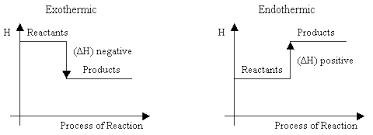
\includegraphics[scale=1]{energyprofile}
\end{center}
\paragraph{The minimum energy to break bonds in order to begin a reaction is the Activation Energy(E$_a$).}
\begin{center}
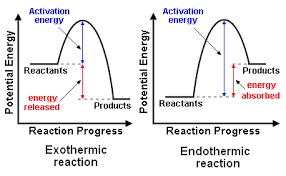
\includegraphics[scale=1]{activationenergy}
\end{center}
\paragraph{These are the standard conditions}needed for physical measurements such as enthalpy changes:
\begin{itemize}
\item Std. pressure: 100 kPa
\item Std. temp : 298K/25$\degree$C
\item Std. states: state that the chemical is in under these conditions.
\end{itemize}
formation,neutralisation,combustion
\paragraph{The enthalpy change of formation}is the enthalpy change that takes place when \textbf{1 mole} of a compound is \textbf{formed} \textbf{from} its \textbf{elements} in their \textbf{standard} states, under standard conditions.
\paragraph{The enthalpy change of combustion}is when \textbf{1 mole} of a \textbf{fuel} \textbf{fully reacts} with \textbf{oxygen} to form CO2 and H2O under \textbf{standard conditions} with all reactants and products in \textbf{std. states}.
\paragraph{The enthalpy change of neutralisation}is when \textbf{1 mole of water} is formed from the reaction of an \textbf{acid and an alkali} under standard conditions with all reactants and products in their \textbf{standard states}.
\begin{itemize}
\item  :\ch{Mg_{(s)} + 1/2 O2_{(g)}-> MgO_{(s)}} :formation
\item \ch{C4H10_{(g)} + 13/2 O2_{(g)} -> 4 CO2_{(g)} + 5H2O{(l)}}: combustion
\item \ch{H^+_{(aq)} + OH^-_{(aq)} -> H2O_{(l)}}: ionic for neut.
\item \ch{HCl_{(aq)} + NaOH_{(aq)} -> H2O_{(l)} + NaCl{(aq)} }
\end{itemize}
\subsection*{Bond enthalpies}
\subsubsection*{Average bond enthalpies}
\paragraph{Average bond enthalpy}is the amount of energy required to break \textbf{one mole} of a \textbf{specified} type of \textbf{bond} in a \textbf{gaseous} \textbf{molecule}. They are \textbf{always endothermic}- therefore values are +ve, but enthalpy of reaction can be -ve.
\paragraph{Bond breaking is endothermic, bond forming is exothermic.} The difference between the two determines if a reaction is exo/endothermic i.e. in an exothermic reaction, there would be more bond forming than bond breaking.
\begin{equation}
\Delta_rH= \Sigma(bond- enthalpies- reactants)-\Sigma(bond- enthalpies- products)
\end{equation}
\begin{center}
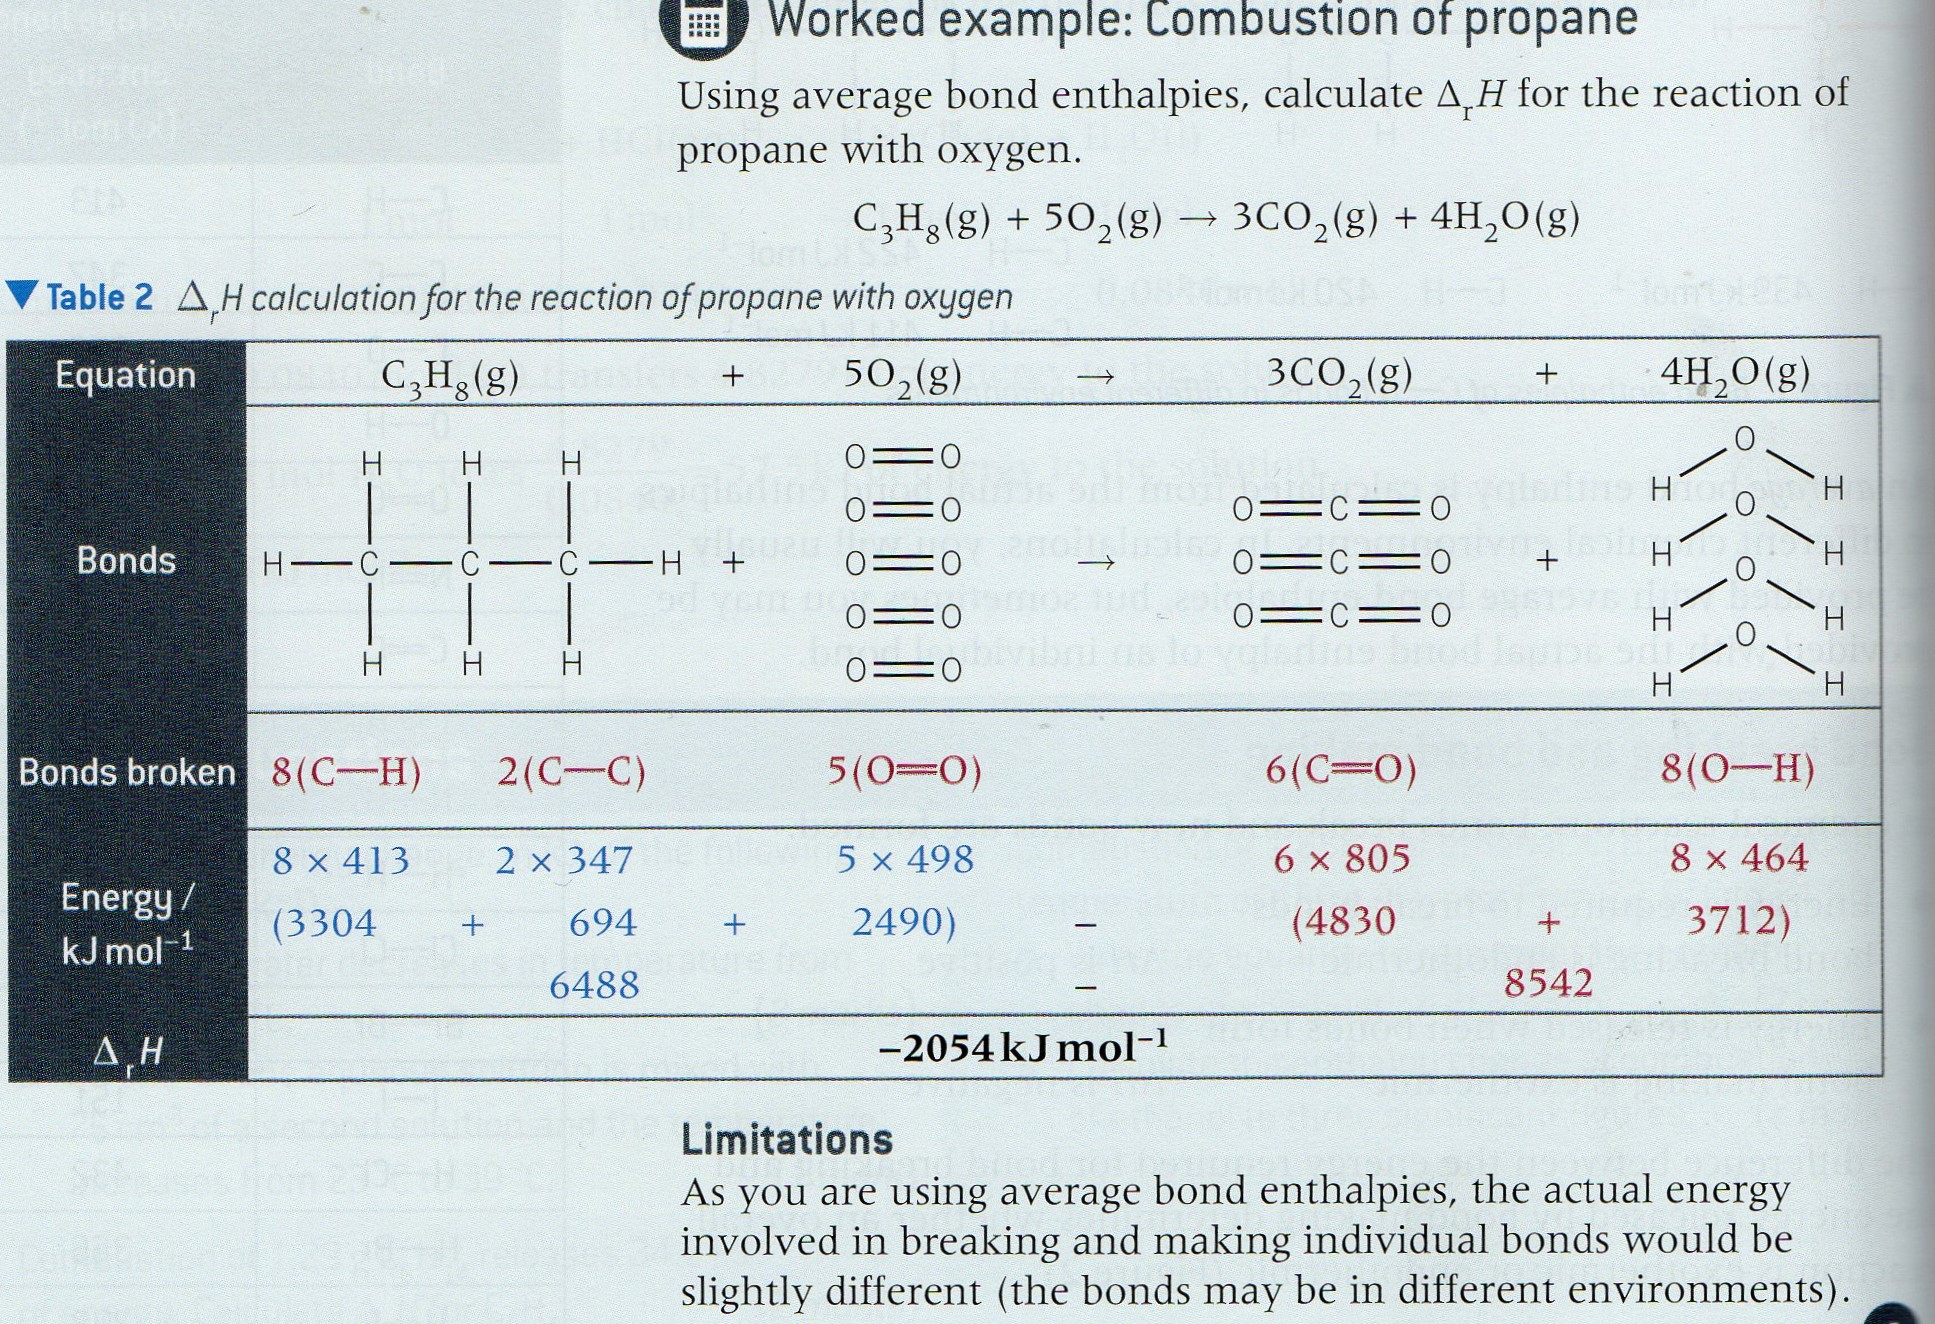
\includegraphics[scale=1]{avgbond}
\end{center}
\subsection{Hess' law and enthalpy cycles}
\paragraph{Hess' law allows enthalpy changes to be found indirectly.}It states that if a reaction can take place by 2 routes, and start and end conditions are the same, the enthalpy. It comes from the idea of conservation of energy.
\paragraph{You need to remember for}enthalpy change of \textbf{formation} \textbf{A+B=C} and for enthalpy change of \textbf{combustion}, \textbf{C+A=B}., where A is from reactant to product, B is elements to reactants and C is elements to product.
\newpage
\begin{center}
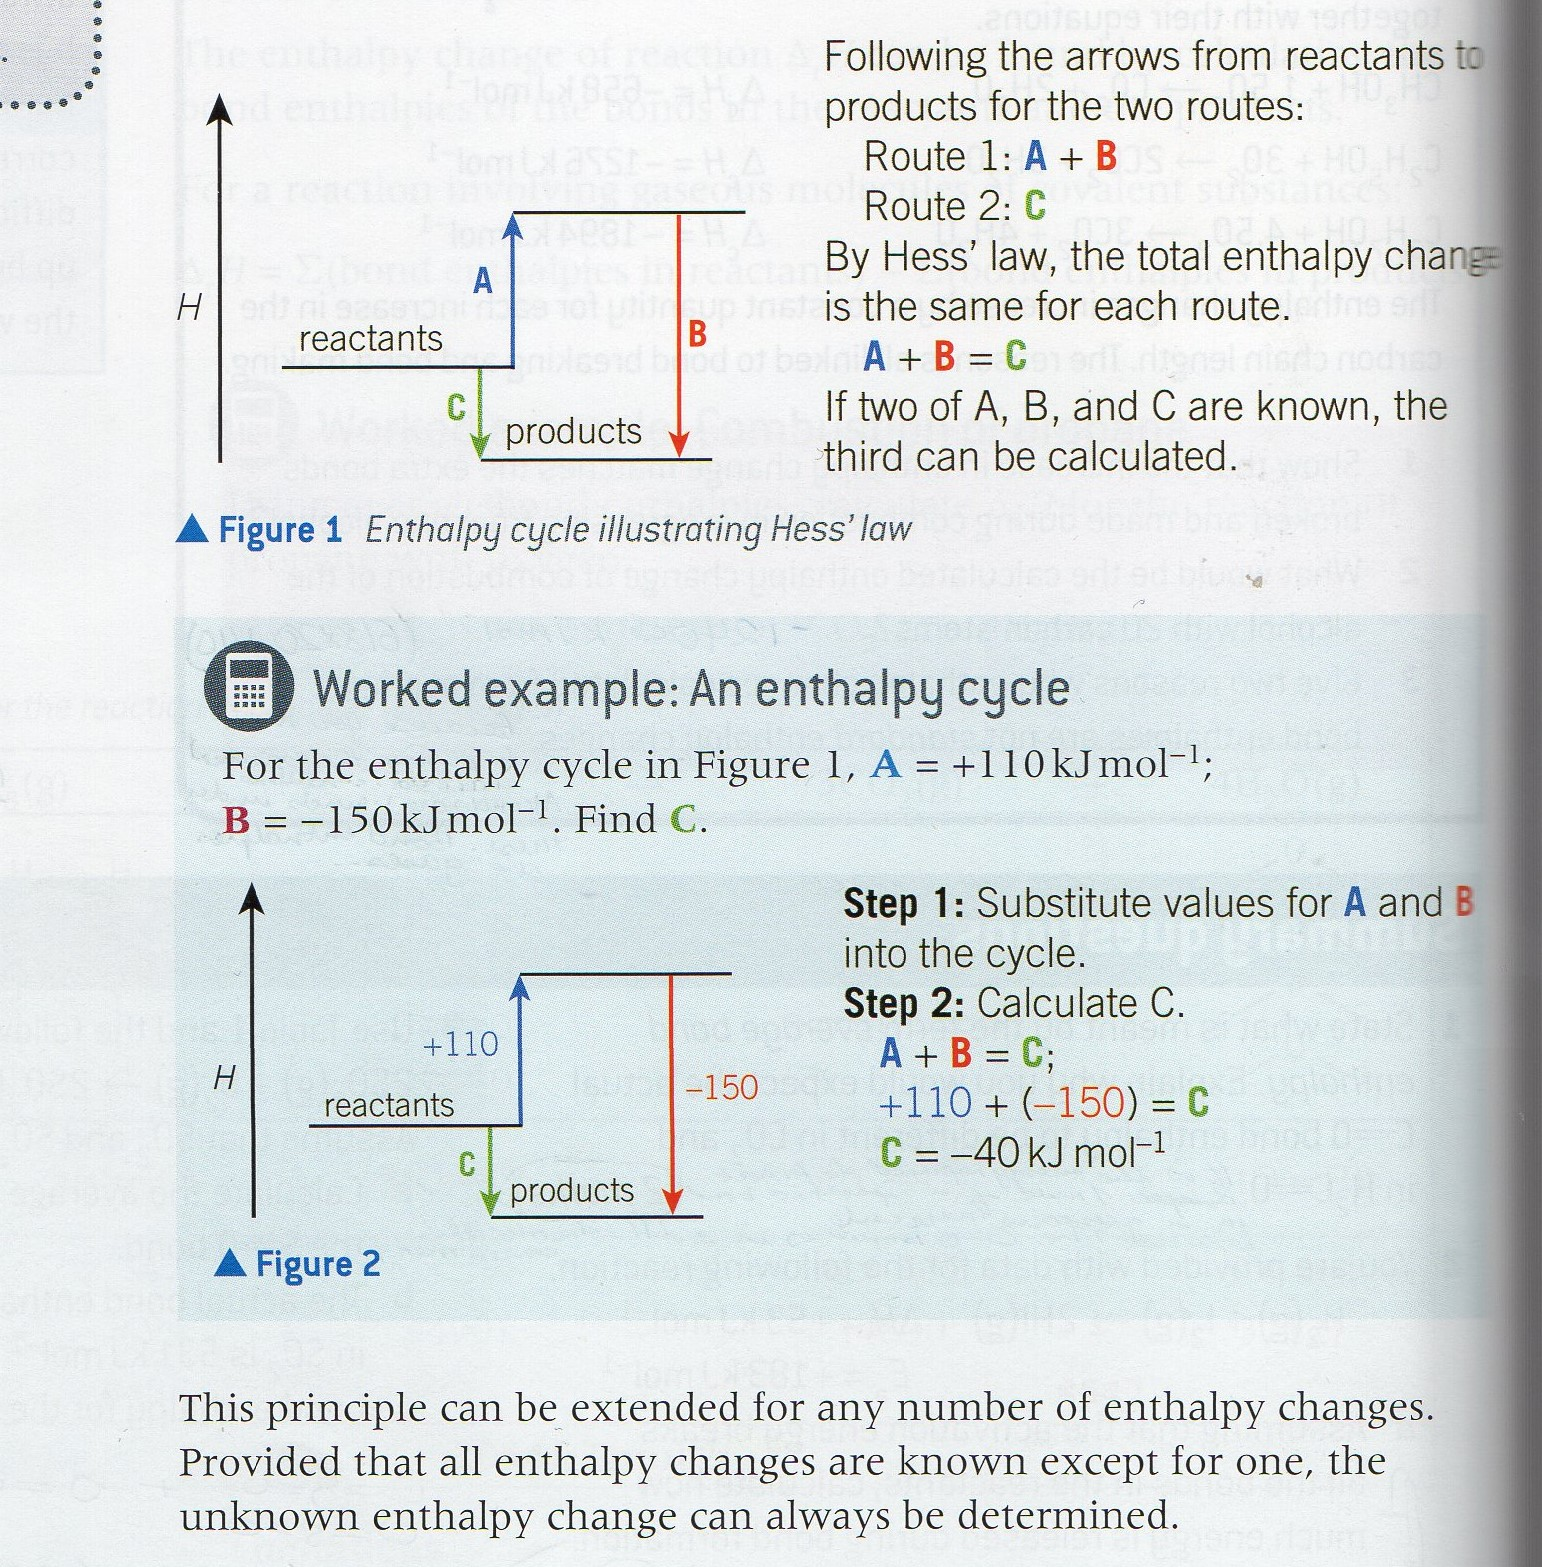
\includegraphics[scale=1]{cycles}
\end{center}


\section{Rates of Reaction 3.2.2}
	\paragraph{Collision} theory hasn't changed at all from GCSE.
	Sill we look at the microscopic consequences of pressure, concentration and temperature (kinetic energy) on individual molecules.
	Successful collisions are needed which is when the reactive atoms in a molecule collide.
	
	\paragraph{Catalysts} are substances that, when added to a chemical reaction, serve to increase the rate of reaction without reacting itself.
	
	This effect is achieved by the catalyst decreasing the required activation energy, thus providing a faster pathway for the reaction to take place.
	
	\paragraph{Homogeneous catalysts} refers to a catalyst that is in the same state as the reactants.
	This works by forming intermediate products.
	
	\paragraph{Heterogeneous catalysts} are catalysts which differ in state from the reactants.
	These act by a series of absorption and desorption.
	
	\paragraph{Catalysts} have massive importance in industry.
	They are used to reduce the amount of energy (in heat and pressure) in industrial reactions.
	This then reduces the amount of fossil fuels needing to be burnt, thus reducing \ch{CO2}.
	
	\paragraph{Measuring} rates of reaction can be done in many ways. This can involve measuring gas or mass over time.
	
	\paragraph{The Boltzmann distribution} is a frequency distribution used to predict the energy of molecules.
	The area under the curve represents the number of molecules with a given energy.
	The curve changes when the temperature rises (skews negativity). E$_a$ moves to the left when a catalyst is added.
	
\section{Chemical equilibrium 3.2.3}

	\paragraph{A dynamic equilibrium} exists in a closed system when the rate of the forward reaction is equal to the rate of the reverse reaction and the concentrations of reactants and products do not change.
	
	\paragraph{le Chatelier’s principle} states that ``When any system at equilibrium is subjected to change in concentration, temperature, volume, or pressure, then the system readjusts itself to (partially) counteract the effect of the applied change and a new equilibrium is established."
	
	Remember that catalysts do not affect the position of equilibrium as they only affect the activation energy, and the reaction goes both ways so this cancels out.
	
	\paragraph{Investigating equilibrium with concentration} is done by the following,
	
	\begin{center}
		\ch{2 CrO4^{2-}(aq) + 2 H^+(aq) <=> Cr2O7^{2-}(aq) + H2O(l)}
	\end{center}
	This reaction is sensitive to the acid concentration. Adding acid concentration will shift the point of equilibrium to the 'right'.
	We can see this because \ch{CrO4^{2-}(aq)} solution is yellow and \ch{Cr2O7^{2-}(aq)} solution is yellow.
	So by raising the concentration of the acid we see the solution got from yellow to orange.
	Procedure is as follows:
	\begin{enumerate}
		\item Add a solution of yellow potassium chromate to a beaker
		\item Add dilute sulfuric acid drop by drop until there is no further change in colour (orange).
		\item Add aqueous sodium hydroxide until there is no further change in colour (yellow).
	\end{enumerate}
	You have now witnessed equilibrium in action.
	\paragraph{Investigating equilibrium with temperature} is done by the following,
	
	\begin{center}
		\ch{[Co(H2O)6]^{2+}(aq) + 4 Cl^-(aq) <=> CoCl4^{2-}(aq) + 6 H2O(l)}
	\end{center}
	As temperature increases the reaction shifts right (in the endothermic direction) and vice-versa. This reaction can be done by the following steps,
	
	\begin{enumerate}
		\item Dissolve cobalt chloride in a boiling tube. Add a small quantity of hydrochloric acid. Then put the solution in ice to cool it until it turns pink (because \ch{[Co(H2O)6]^{2+}(aq)} solution is pink).
		\item Set up a boiling water bath and transfer the boiling tube. Wait until it turns blue (because \ch{CoCL4^{2-}} is blue).
		\item Transfer back to ice water and observe the change back to pink.
	\end{enumerate}
	And you have now witnessed a shift in equilibrium.
	
\section{The equilibrium constant, $K_c$ 3.2.3}

	\paragraph{Equilibrium constant} is calculated by,
	\begin{center}
		In the reaction $a$A + $b$B \ch{<=>} $c$C + $d$D
		\begin{equation}
			K_c = \frac{[\textnormal{C}]^c[\textnormal{D}]^d}{[\textnormal{A}]^a[\textnormal{B}]^b}
		\end{equation}
	\end{center}
	This requires a little explaining, The A, B, C and D values are the \textit{equilibrium} concentrations of the reactants (in mol dm$^{-3}$).
	
	Where $K_c = 1$ it indicates that the reaction is halfway between reactants and products.
	
	Where $K_c > 1$ it indicates that the position of equilibrium is shifted to the right (the products).
	
	Where $K_c < 1$ it indicates that the position of equilibrium is shifted to the left (the reactants).
	